\documentclass[a4paper,12pt]{article}
\usepackage[margin=1in]{geometry}

\usepackage[T2A]{fontenc}			% кодировка
\usepackage[utf8]{inputenc}			% кодировка исходного текста
\usepackage[english,russian]{babel}	% локализация и переносы
\usepackage{graphicx}                % Математика
\usepackage{amsmath,amsfonts,amssymb,amsthm,mathtools} 
\usepackage{mathtext}
\usepackage[T2A]{fontenc}
\usepackage[utf8]{inputenc}
\usepackage{multirow}

\usepackage{wasysym}

%Заговолок
\author{Бичина Марина 
группа Б04-005 2 курса ФЭФМ}
\title{}
\date{}


\begin{document} % начало документа

\begin{center}
\begin{Large}
{Корнеев Николай Б04-005, Лабораторная работа №. 4.3.3 <<Исследование разрешающей способности микроскопа методом Аббе>>}
\end{Large}
\end{center}
\subsection*{Цель работы:} 
Определение дифракционного предела разрешения объектива микроскопа методом Аббе
\paragraph{Задание:} 
\begin{enumerate}
\itemsep0em
\item Определить периоды сеток
\begin{enumerate}
\itemsep0em
\item по их спектру на удаленном экране
\item по увеличенному с помощью модели микроскопа изображению сеток на экране
\item по результатам измерения разрешающей способности микроскопа
\end{enumerate}
\item наблюдать явление саморепродукции
\item наблюдать явление пространственной фильтрации 
\item наблюдать явление мультиплицирования
\end{enumerate}
\subsection*{Оборудование:}
\begin{enumerate}
\itemsep0em
\item лазер
\item кассета с набором сеток разного периода
\item линзы
\item щель с микрометрическим винтом
\item оптический стол с набором рейтеров и крепежных винтов
\item экран
\item линейка
\end{enumerate}
\subsection*{Теоретическая справка:}
\paragraph{Разрешающая способность:}
Любая оптическая система имеет конечный предел разрешения. Принципиальной причиной, ограничивающей предел разрешения, является дифракция световых волн. \\
Визуально, в качестве критерия разрешения применяют критерий Рэлея.\\
Для иммерсионного микроскопа разрешающая способность при некогерентном освещении 
\begin{equation}
l_{min} \approx \frac{0.61\lambda}{n\cdot \sin A}
\end{equation}
где:\\  
$n$ -- коэффициент приломления\\
$A$ -- апертурный угол объектива микроскопа\\
При когерентном освещении формула принимает вид \begin{equation}
l_{min} \approx \frac{0.61\lambda}{n\cdot \sin A} \approx \frac{\lambda}{D/2f}
\end{equation}
где $D$ -- диафрагма
\paragraph{Дифракция Фраунгофера на двумерной решетке}
При дифракции Фраунгофера на решетке периода d направления $\theta$ максимумы интенсивности определяются из условия
\[d\sin\theta = m\lambda\] 
Двумерную решетку можно рассматривать как две перпендикулярные друг другу, для максимумов которых выполняется соотношение:
\begin{equation}
d\sin \theta_{x} = m_{x}\lambda, \;\;\;\;\;\;\;\;\;\;\;\; d\sin\theta_{y} = m_{y}\lambda
\end{equation}
где \\
$\theta_{x}, \;\; \theta_{y}$ -- направления на главные дифракционные
максимумы в горизонтальной и вертикальной плоскостях соответственно\\
$m_{x}, \;\; m_{y}$ -- целые числа, характеризующие порядок дифракционных максимумов
\begin{figure}[h!]
\centering
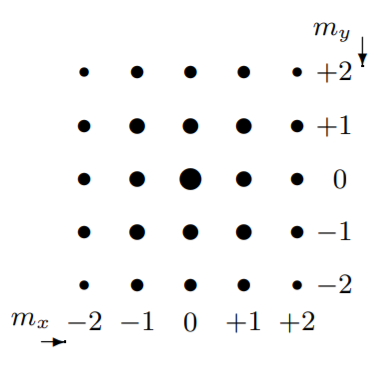
\includegraphics[scale=0.5]{FG.png} 
\caption{Дифракция Фраунгофера. Максимумы изображены кружками, размеры которых характеризуют интенсивности.}
\end{figure}
\paragraph{Описание установки:}
\begin{enumerate}
\itemsep0em
\item Установка для 1 пункта
\begin{figure}[h!]
\centering
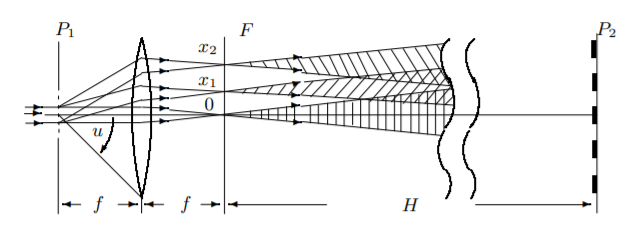
\includegraphics[scale=0.8]{setup_0.png}
\caption{Изображение в объективе микроскопа} 
\end{figure}
\item Установка для 2 пункта\\
\begin{figure}[h!]
\centering
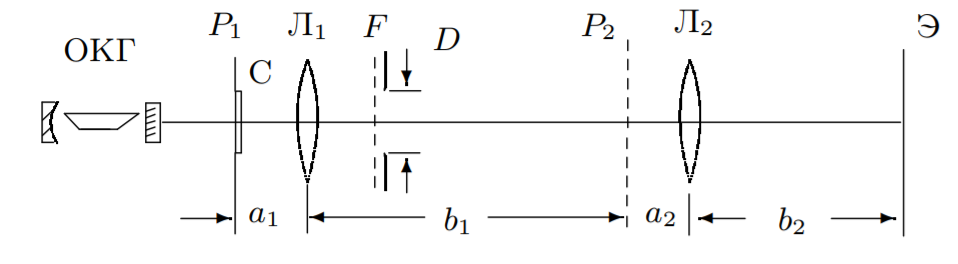
\includegraphics[scale=0.5]{setup.png}
\caption{Схема экспериментальной установки -- модель проекционного микроскопа} 
\end{figure}
ОКГ -- лазер\\
С -- сетка\\
Л$_1$ -- объектив микроскопа $F_1 = 100$ мм\\
Л$_2$ -- линза 2 $F_2 = 25$ мм\\
$P_1$ -- плоскость предмета\\
$P_2$ -- плоскость вторичного изображения\\
Э -- экран\\
D -- диафрагма (находится в фокальной плоскости F)
\end{enumerate}
\subsection*{Ход работы:}
\paragraph{Определение периода решеток по их пространственному спектру}
\begin{enumerate}
\itemsep0em
\item Соберем установку, как показано на рисунке 2
\item  Пронаблюдаем на удаленном экране дифракционные картины для разных сеток
\item Измерим расстояние между удаленными друг от друга максимумами и число промежутков между ними.\\
Запишем расстояние от сетки до экрана $H = 1380$ мм. Рассчитаем период решетки по формуле:
\[ d = \frac{\lambda H(n-1)}{x_{n}}\]
где\\ $x_{n}$ -- расстояние между n максимумами.\\
x - расстояние между соседними максимумами
\item Расчитаем погрешность  для d по формуле:
\[\sigma_{d} = d\sqrt{\left(\frac{\sigma_{x} }{x_{n}}\right)^2+ \left(\frac{\sigma_{H}}{H}\right)^2} \]
При измерении расстояния между максимумами учтем погрешность линейки (0.5 мм) и толщину пятна $\Delta \approx 4$ мм. Так толщина пятна в 8 раз больше погрешности линейки, будем считать погрешность измерений $\sigma_{x} = \Delta\sqrt{2}\approx 3$ мм (2 пятна с разных концов).\\
Так как невозможно точно измерить положение сетки в кассете, будем считать погрешность примерно равной толщине кассеты, т.е. 10 мм.
\[\sigma_{d} = d\sqrt{\left(\frac{3\;\;\text{мм}}{x_{n}}\right)^2 + 5\cdot 10^{-5}}\]
\item Сведем данные в таблицу для каждой сетки 
\begin{table}[h!]
\centering
\begin{tabular}{|c|c|c|l|c|c|c|c|c|}
\hline
N сетки & n, ед & $x_{n}$, мм & x, мм & $\sigma_{x}$, мм   & H, мм                 & $\varepsilon_{H}$                 & d, мкм & $\sigma_d$, мкм \\ \hline
1       & 2     & 76          & 38    & \multirow{5}{*}{3} & \multirow{5}{*}{1380} & \multirow{5}{*}{$5\cdot 10^{-5}$} & 19     & 0.76            \\ \cline{1-4} \cline{8-9} 
2       & 2     & 51          & 25.5  &                    &                       &                                   & 29     & 1.71            \\ \cline{1-4} \cline{8-9} 
3       & 3     & 39          & 13    &                    &                       &                                   & 56     & 4.33            \\ \cline{1-4} \cline{8-9} 
4       & 8     & 50          & 6.25  &                    &                       &                                   & 117    & 7               \\ \cline{1-4} \cline{8-9} 
5       & 13    & 61          & 4.69  &                    &                       &                                   & 156    & 7.75            \\ \hline
\end{tabular}
\caption{Периоды решеток с помощью метода пространственного спектра}
\end{table} 
\end{enumerate}
\paragraph{Определение периода решеток по изображению, увеличенному с помощью модели микроскопа}
\begin{enumerate}
\itemsep0em
\item Соберем установку, как показано на рисунке 3. Отцентрируем систему. Измерим необходимые расстояния. 
\[a_1 = 140 \pm 10\;\; \text{мм}\]
\[a_2 + b_1 = 870 \pm 10\;\; \text{мм}\]
\[b_2 = 40 \pm 10\;\; \text{мм}\]
Учтем, что $a_2\approx F_2\approx 25 \;\;\text{мм}$, так что $b_1 = 845 \pm 10 \;\;\text{мм}$
\item Рассчитаем увеличение микроскопа по формуле:
\[\Gamma = \frac{b_1b_2}{a_1a_2} \approx 96.6\]
\item Так как определить точное расстояние между центрами линз невозможно из-за широкой оправы, будем считать погрешность измерения расстояний по ширине оправы $\sigma_{x}\approx 10$ мм, $a_2$ берем без погрешности, так как считаем его разным фокусному расстоянию $F_2$.  
\item Рассчитаем погрешность увеличения:
\[\sigma_{\Gamma} =\Gamma \sqrt{\left(\frac{\sigma_{x}}{ a_1}\right)^2 + \left(\frac{\sigma_{x}}{b_1}\right)^2+ \left(\frac{\sigma_{x}}{ b_2}\right)^2}\approx 7\]

\item На экране измерим расстояние между максимумами разных порядков 
 
Для каждой дифракционной решётки получим её увеличенное изображение. Заметим, что полученное изображение искажено по краям, это связанно с геометрией линзы. В пределах мало искажённого участка изображения ($\approx \pm 5$ см от оптической оси) измерим расстояние $x_n$ между краями $n$ клеток, и ширину решётки $\delta x$. Рассчитаем период решётки и погрешность по формуле:

\[
d = \frac{x_n}{n \Gamma}, \;\;\; \sigma_d = d \cdot \sqrt{\left( \frac{\sigma_x}{x_n} \right) ^ 2 + \left( \frac{\sigma_\Gamma}{\Gamma} \right) ^ 2 } = d \cdot \sqrt{\left( \frac{\sigma_x}{x_n} \right) ^ 2 + 5 \cdot 10^{-3} }.
\]

\noindent В качестве погрешности $\sigma_x$ возьмём значения $\delta x$ так как они больше погрешности линейки, кроме случая для первой решётки.
\item Полученные результаты сведем в таблицу:
\begin{table}[]
\centering
\begin{tabular}{|l|l|l|l|l|l|l|}
\hline
$N$ сетки & $n$ ед & $x_n$, мм & $\delta x$,  мм & $x$, мм & $d$, мкм & $\sigma_d$, мкм \\ \hline
1   & 30  & 44        & --              & 1.5     & 15.2     & 1.1             \\ \hline
2   & 30  & 65        & 1              & 2.2     & 22.4     & 1.6             \\ \hline
3   & 15  & 101       & 1              & 6.7     & 69.7     & 5.0             \\ \hline
4   & 6   & 79        & 3              & 13.2    & 136      & 11              \\ \hline
5   & 6   & 102       & 4              & 17.0    & 156      & 14              \\ \hline
\end{tabular}
\caption{Периоды решеток по изображению, увеличенному с помощью модели микроскопа}
\label{tab:2met}
\end{table}
\end{enumerate}
\paragraph{Определение периодов микроскопа по оценке разрешающей способности микроскопа}
\begin{enumerate}
\itemsep0em
\item Расположим в фокальной плоскости длиннофокусной линзы диафрагму в соответствии с рисунком 3.  
\item Для каждой решетки определим минимальный размер диафрагмы D, при котором еще различима картинка сетки.
\item По формуле 2  вычислим период решетки. Оценить точность такого метода сложно, так как превращение изображения сетки в изображение полос происходит плавно и для разных решеток -- с разной скоростью.
\item Сведем полученные данные в таблицу
\begin{table}[h!]
\centering
\begin{tabular}{|l|l|l|}
\hline
$N$ сетки & $D$, мкм & $d$, мкм \\ \hline
1   & --        & --        \\ \hline
2   & 4140     & 28.27       \\ \hline
3   & 1960     & 59.7      \\ \hline
4   & 1020     & 114.7      \\ \hline
5   & 810      & 144.5      \\ \hline
\end{tabular}
\caption{Периоды решеток, полученные по оценке разрешающей способности микроскопа}
\label{tab:3met}
\end{table} 
\item Для проверки теории Аббе построим график зависимости $d = f(1/D)$, взяв периоды сеток определённые по спектру. Проведём прямую по МНК для наглядности.
\begin{equation*}
b = \frac{\langle xy \rangle - \langle x \rangle \langle y \rangle}{\langle x^2 \rangle - \langle x \rangle^2} \;\;
a = \langle y \rangle - b \cdot \langle x \rangle
		\end{equation*}
\begin{figure}[h!]
\centering
\includegraphics[scale=0.8]{../../../../../Users/Marina/plot_4_3_3.png} 
\end{figure}
\item Видим, что четыре точки действительно образуют прямую, проходящую через начало координат (с некоторой погрешностью). Учитывая то, что значения для периода сетки полученные по оценке разрешающей способности близки к значениям полученными другими способами, можно сделать вывод, что теория Аббе работает в условиях этого эксперимента.\\
Также, коэффициент наклона графика, равный $k = (124 \pm 8)\cdot 10^{-9}$ м$^2$ в пределах погрешности совпадает с $2\lambda F_1 = 117\cdot 10^{-9}$ м$^2$
\end{enumerate}
\paragraph{Пространственная фильтрация и мультиплицирование}
\begin{enumerate}
\itemsep0em
\item
\textbf{Пространственная фильтрация.} Пропуская только вертикальные дифракционные максимумы, получим на экране картинку горизонтальных полос, находящихся на расстоянии равном увеличенному периоду решётки друг от друга. При пропускании только горизонтальных максимумов, получим такие же полосы, но расположенные вертикально.\\ Пропуская только диагональные максимумы, получим изображение решётки с периодом, увеличенным в $\sqrt{2}$ раз. 
\item
\textbf{Мультиплицирование.} Расположив щель за дифракционной решёткой, получим множество изображений щелей, повторяющихся периодически по горизонтали и вертикали.
\end{enumerate}
\subsection*{Выводы:}
\begin{enumerate}
\itemsep0em
\item Нашли периоды дифракционных решёток тремя способами и получили следующие значения:
\begin{table}[h!]
\centering
\begin{tabular}{|c|cc|cc|c|}
\hline
        & \multicolumn{2}{c|}{1 способ}                  & \multicolumn{2}{c|}{2 способ}                   & 3 способ \\ \hline
N сетки & \multicolumn{1}{c|}{d, мкм} & $\sigma_{d}$ мкм & \multicolumn{1}{c|}{d, мкм} & $\sigma_{d}$, мкм & d, мкм   \\ \hline
1       & \multicolumn{1}{c|}{19}     & 0.76             & \multicolumn{1}{c|}{15.2}   & 1.1               & --       \\ \hline
2       & \multicolumn{1}{c|}{29}     & 1.71             & \multicolumn{1}{c|}{22.4}   & 1.6               & 28.27    \\ \hline
3       & \multicolumn{1}{c|}{56}     & 4.33             & \multicolumn{1}{c|}{69.7}   & 5                 & 56.7     \\ \hline
4       & \multicolumn{1}{c|}{117}    & 7                & \multicolumn{1}{c|}{136}    & 11                & 114.7    \\ \hline
5       & \multicolumn{1}{c|}{156}    & 7.75             & \multicolumn{1}{c|}{156}    & 14                & 144.5    \\ \hline
\end{tabular}
\end{table}
\item Основываясь на полученных данных проверили теорию Аббе

\item Пронаблюдали качественно эффекты пространственной фильтрации и мультиплицирования.
\end{enumerate}
\end{document}